% utk buat flowchart guna TikZ
\documentclass{minimal}

\usepackage{tikz}

\usetikzlibrary{shapes, arrows, positioning}

\begin{document}

Usual way to connect nodes with path

\hfill

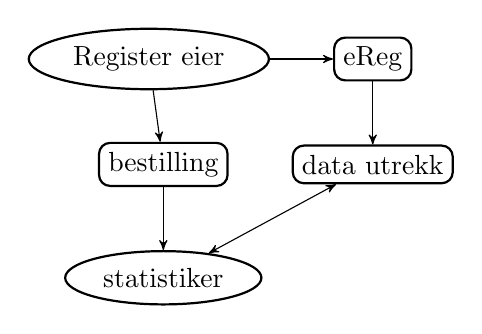
\begin{tikzpicture}
  [
  % block
  block/.style = {rectangle,
    rounded corners,
    draw, thick,
    node distance = 8mm,
    minimum height = 2mm},
  %bulat
  bulat/.style = {ellipse,
    draw, thick, node distance = 8mm,
    minimum height = 5mm},
  % line
  line/.style = {draw, -stealth'},
  ]

  % nodes
  \node [block] (ereg) {eReg};
  \node [bulat, base left= of ereg] (eier) {Register eier};
  \node [block, below= of ereg] (ut) {data utrekk};
  \node [block, left= of ut] (bestil) {bestilling};
  \node [bulat, below= of bestil] (stat) {statistiker};

  % Hvordan får man to noder på lik linje?

  % path
  \path [line] (eier) -- (ereg);
  \path [line] (ereg) -- (ut);
  \path [line] (eier) -- (bestil);
  \path [line] (bestil) -- (stat);
  \path [line, <->, >=stealth'] (ut) -- (stat);

\end{tikzpicture}

\hfill

Arrow under ellipse to rectangle with \textbf{\texttt{-|}} as path ID

\hfill

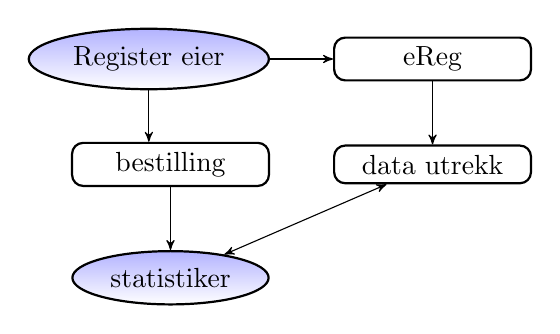
\begin{tikzpicture}
  [
  % block
  block/.style = {rectangle,
    rounded corners,
    draw, thick,
    node distance = 8mm,
    minimum height = 2mm,
    minimum width = 2.5cm},
  %bulat
  bulat/.style = {ellipse,
    draw, thick, node distance = 8mm,
    minimum height = 5mm, top color=blue!30},
  % line
  line/.style = {draw, -stealth'},
  ]

  % nodes
  \node [block] (ereg) {eReg};
  \node [bulat, base left= of ereg] (eier) {Register eier};
  \node [block, below= of ereg] (ut) {data utrekk};
  \node [block, left= of ut] (bestil) {bestilling};
  \node [bulat, below= of bestil] (stat) {statistiker};

  % Hvordan får man to noder på lik linje?

  % path
  \path [line] (eier) -- (ereg);
  \path [line] (ereg) -- (ut);
  \path [line] (eier) -- (bestil.north -| eier.south); % specify intersection
  \path [line] (bestil) -- (stat);
  \path [line, <->, >=stealth'] (ut) -- (stat);

\end{tikzpicture}

\hfill

In case someone needs it, this syntax is explained in pgfmanual section "13.3.1 Intersections of Perpendicular Lines".

\texttt{(<p> |- <q>) or (<q> -| <p>)} represent a coordinate at intersection point
between a vertical line passing through coordinate \verb|<p>| and an horizontal
passing through \verb|<q>|. You can use named coordinates like
\texttt{(bestil.north |- eier.south)} that is used here or numeric pairs like in \texttt{(2,1 |- 3,4)}.

\hfill

To get alle the nodes aligned for both ellipse and rectangle, the structure starts
from the middle i.e \texttt{bestil} and specify the direction from there.

\hfill

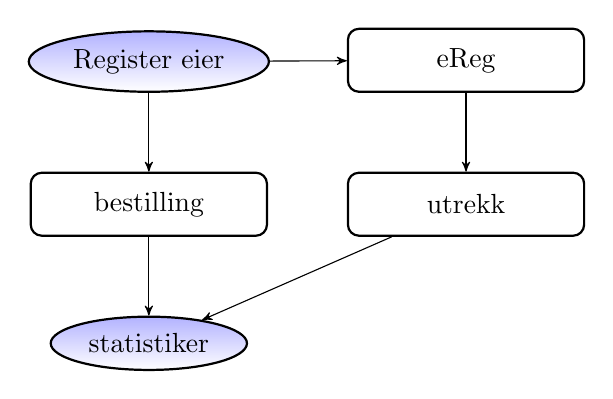
\begin{tikzpicture}
  [
  block/.style = {rectangle, rounded corners,
    draw, thick, node distance = 1cm, minimum height = 8mm,
    minimum width = 3cm},
  % bulat
  bulat/.style = {ellipse,
    draw, thick, node distance = 1cm,
    minimum height = 5mm, top color=blue!30},
  % line
  line/.style = {draw, -stealth'},
  node distance = 2cm,
  ]

  % nodes
  \node [block] (bestil) {bestilling};
  \node [bulat, above= of bestil] (eier) {Register eier};
  \node [block, right= of bestil] (ut) {utrekk};
  \node [block, above= of ut] (ereg) {eReg};
  \node [bulat, below= of bestil] (stat) {statistiker};

  % path
  \path [line] (eier) -- (bestil);
  \path [line] (ereg) -- (ut);
  \path [line] (eier) -- (ereg);
  \path [line] (bestil) -- (stat);
  \path [line] (ut) -- (stat);

\end{tikzpicture}

\end{document}
